\section{Results}

To validate the PIC portion of SINATRA, two main methods have been used: Solver Validation and Test Cases. By both testing the individual solver as well as comparing test cases to literature, SINATRA's new upgrade can be trusted as an accurate PIC code for it's methods. All input files used for the test cases can be found in Appendix \ref{app:validation_input}. The top of each page of that appendix shows the title of the test case. That same title will be bolded in the thesis writing. All simulations can be run using the master branch in GitHub\textsuperscript{\textregistered}, version committed on June 14\textsuperscript{th}, 2019 or later.

\subsection{Solver Validation}

In order to validate that the Gauss-Sidel solver, the important components of the solver were logged during operation. Then the same inputs were put into a heritage validated Gauss-Seidel solver. This solver was run to the same tolerance. The results of the two solvers were then compared to confirm that SINATRA's solver is valid. \par




\indent A more visual way to confirm that the solver works is by observing the error as the iterations increase. A few tests were run and the error of the solver were outputted at each iteration. A simple 8 cell version is shown in Figure \ref{fig:error8} and a larger 4096 cell version is shown in Figure \ref{fig:error4096}. As seen in these figures, the iterative solver reduces the error in the simulation quickly to below the required tolerance. 


\begin{figure}
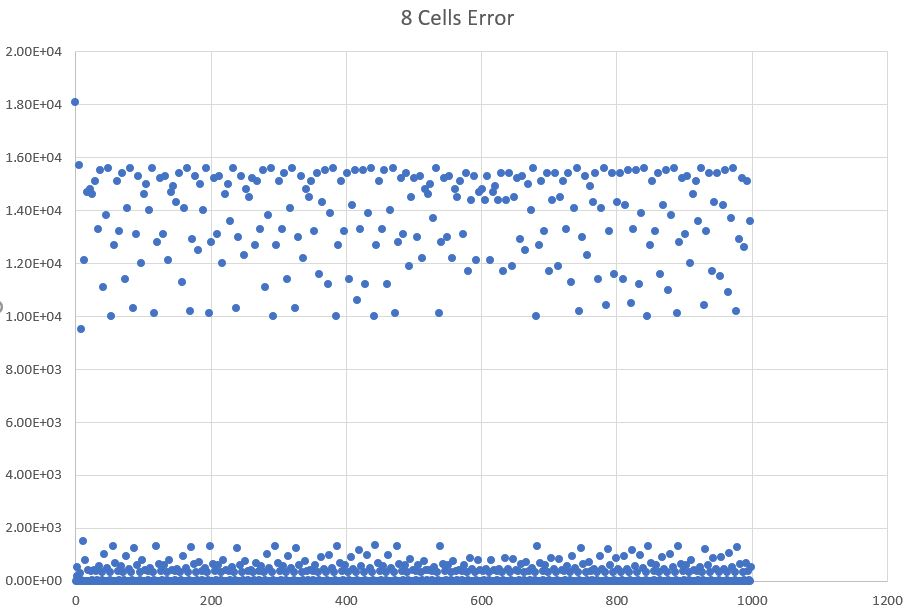
\includegraphics[width=.95\textwidth]{figures/error8.JPG}
\centering
\caption{Error of the Gauss-Seidel solver over 1000 iterations for 8 cells}
\label{fig:error8}
\end{figure}


\begin{figure}
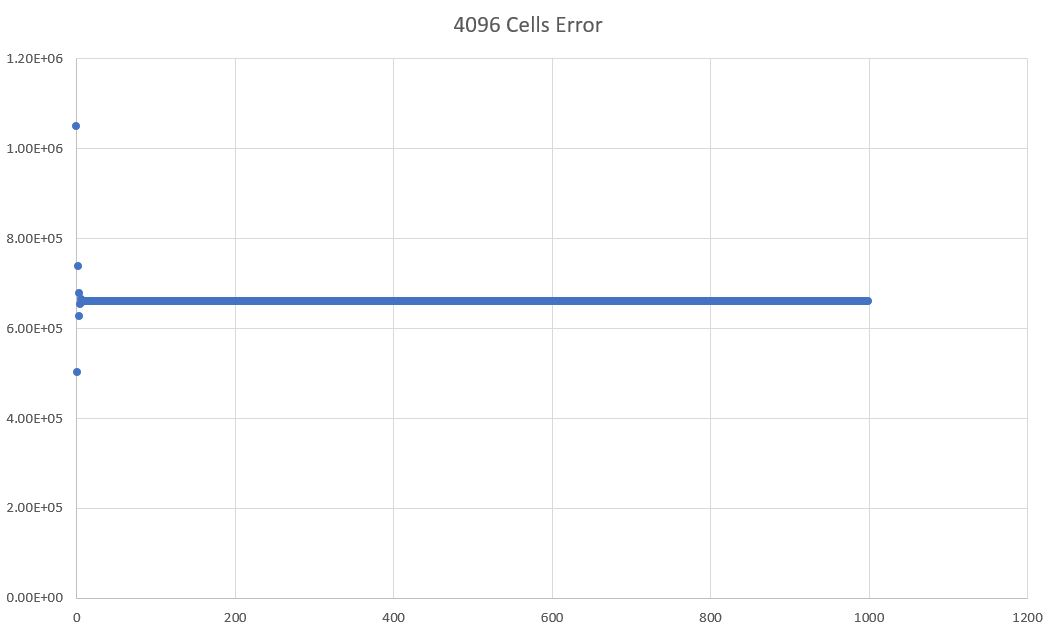
\includegraphics[width=.95\textwidth]{figures/error4096.JPG}
\centering
\caption{Error of the Gauss-Seidel solver over 1000 iterations for 4096 cells}
\label{fig:error4096}
\end{figure}


\subsection{Test Cases}

Two main test cases were performed in order to test the validation of the SINATRA: Ambipolar diffusion and Collette flow. Ambipolar diffusion is a typical simulation case for PIC codes. Normal fluids will diffuse out of a domain naturally over time. However, on account of the different speeds between electrons and ions in a plasma, a gradient is set up as the electrons start to move faster than the ions. This gradient causes an electric field which in turn reduces the speed of the electrons while increasing the speed of the ions. This causes a uniform diffusion rate. A comparison between a charged simulation diffusion and neutrals is seen in the next 4 figures. \par

Simulations were not doing anything physical, therefore not included yet. 

\indent Collette flow. (I didn't even simulate these yet until I have the solver converging.)


\subsection{Execution Time Study}

In order to examine the performance hit on SINATRA by adding PIC a execution time study was performed. Simulations were run keeping the same number of particles but changing the mesh size, as well as holding the mesh size and changing the number of particles. It is also compared to a comparable non-charged simulation. The results can be found in Table \ref{tab:pic_time}.

\begin{table}
\caption{PIC Execution Time}
\label{tab:pic_time}
\vspace{0.3cm}
\begin{center}
\begin{tabular}{|l|l|l|l|}
\hline
                             & First Iteration & Timestep Average & Total Time     \\ \hline
Parallel and No Linking & 9 sec           & 10 sec           & 1 min, 38 sec  \\ \hline
Serial and No Linking   & 3 min, 23 sec   & 3 min, 23 sec    & 33 min, 50 sec \\ \hline
Serial and Linking      & 15 min, 1 sec   &  3 min, 58 sec   &   50 min, 47 sec             \\ \hline
\end{tabular}
\end{center}
\end{table}

\indent Through these results it can be seen that the execution time is more heavily influenced by the number of particles than the number of mesh cells. It also shows that parallizationn makes a negligible difference in the PIC code. It is future work to find a much quicker solver in order to increase the simulation accuracy of SINATRA. 
